\chapter{Introduction}
\label{chap:intro}
{\em Written by Ben Kushigian}
\section{What are fractals?}
In what follows we will be investigating fractals and some of their interesting
properties. First we define a fractal.

\begin{dfn}
  A {\bf fractal}\index{fractal} is a curve or geometric figure, each part of
  which has the same statistical character as the whole.
\end{dfn}

\begin{wrapfigure}{r}{0.35\textwidth}
  \centering
  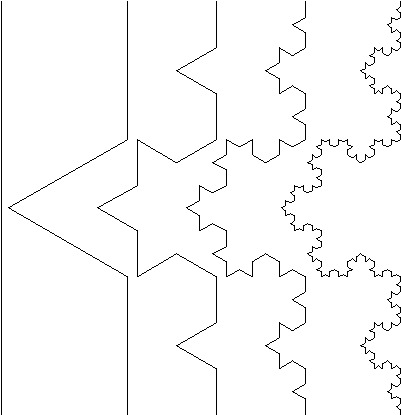
\includegraphics[width=0.33\textwidth]{img/bk_introkochgen}
  \caption{The first few iterations in generating the Koch Curve}
  \label{fig:intro koch}
\end{wrapfigure}

What this means in layterms is that a fractal is a shape or set that has
similar properties at all magnifications. We have a special name for this
property: {\em self similarity}\index{self similar}. A classic example is the
{\em Koch Curve} (Fig \ref{fig:intro koch}) which looks identical at all levels
of magnification. We should note that there are certain degenerate cases which
satisfy our definition such as a straight line. The distinction between a true
fractal and a degenerate case can be made with the notion of {\em fractal
dimension} which we will touch upon in Chapter \ref{chap:measure} which deals
with measure theory.\\

\section{Fractal Generation}
\label{sec:fractal generation}
It is often useful to think of a fractal as a set of points. However it is
often difficult to explicitly state which points are in our fractal. A standard
technique for fractal generation is to describe the {\em generation} of a 
fractal {\em iteratively} or {\em corecursively}. Typically we start with a
base case, usually a set \(A_0\), and define some sort of operation \(\varphi\)
on a set and define \(A_{i+1} = \varphi(A_i)\) for \(i \in \Z^+\). In
Fig \ref{fig:intro koch} we see that our base case is a straight line and our
operation \(\varphi\) replaces the middle third of each line segment in \(A_i\)
with two line segments forming the top part of a triangle.\\

But at what point is our shape a fractal? \(A_0\) obviously is not fractal - 
it is just a line segment and holds no interest for us. Likewise \(A_1\) is
not a fractal since it is just four line segments. What about \(A_{10}\) or
\(A_{100}\)? \(A_{1,000,000}\)? None of these are in fact fractals. They 
{\em appear} to be fractal since we can only see detail larger than a certain
scale. In fact, any fractal you have ever seen has only been an approximation
of a fractal; true fractals are self similar and look the same at all scales.\\

So how is our construction useful? Well at no finite stage have we created a
fractal but we can steal the analytic notion of the limit. First we defined the
distance between a point \(\bm{x} = (x_1,x_2)\) and a set \(S\subset \R^2\) as
\[d(\bm{x},S) = \inf_{\bm{y} \in S}{\{|x-y|\}}.\]
Formally we define the Koch curve as the collection of points \(\bm{x} \in
\R^2\) so that for any given \(\varepsilon > 0\) there exists an \(N > 0\) with
\(d(\bm{x},A_n) < \varepsilon\) for all \(n > N\). \\

We will see in Chapter \ref{chap:complex dynamics} that there are other ways
to generate and define fractals. We should also note that the term fractal is
used in a number of ways. We often refer to shapes in nature as fractal even
though they often bottom out after a finite, often rather low, number of
iterations.
